\documentclass[tikz,border=8pt]{standalone}
% Shared TikZ preamble for book diagrams
% Usage: % Shared TikZ preamble for book diagrams
% Usage: % Shared TikZ preamble for book diagrams
% Usage: \input{../preamble.tex} after \documentclass

\usepackage{tikz}
\usepackage{amsmath,amssymb}

\usetikzlibrary{arrows.meta, calc, positioning, decorations.pathreplacing}

% --- Color palette ---
% Consistent across all diagrams in the book
\definecolor{basis1}{RGB}{31,119,180}    % blue: encoders, structure
\definecolor{msg}{RGB}{44,160,44}        % green: positives
\definecolor{aux}{RGB}{127,127,127}      % gray: alternatives, auxiliary
\definecolor{highlight}{RGB}{255,127,14} % orange: highlights
\definecolor{lightfill}{RGB}{230,240,255}% light blue: shaded regions

% --- Reusable styles ---
\tikzset{
  encoder/.style={draw=basis1!60, fill=lightfill, rounded corners=3pt,
    minimum width=1.0cm, minimum height=0.8cm},
  flow/.style={-{Stealth[length=5pt,width=4pt]}, line width=0.8pt},
  annotation/.style={font=\footnotesize, text=aux!80!black},
}
 after \documentclass

\usepackage{tikz}
\usepackage{amsmath,amssymb}

\usetikzlibrary{arrows.meta, calc, positioning, decorations.pathreplacing}

% --- Color palette ---
% Consistent across all diagrams in the book
\definecolor{basis1}{RGB}{31,119,180}    % blue: encoders, structure
\definecolor{msg}{RGB}{44,160,44}        % green: positives
\definecolor{aux}{RGB}{127,127,127}      % gray: alternatives, auxiliary
\definecolor{highlight}{RGB}{255,127,14} % orange: highlights
\definecolor{lightfill}{RGB}{230,240,255}% light blue: shaded regions

% --- Reusable styles ---
\tikzset{
  encoder/.style={draw=basis1!60, fill=lightfill, rounded corners=3pt,
    minimum width=1.0cm, minimum height=0.8cm},
  flow/.style={-{Stealth[length=5pt,width=4pt]}, line width=0.8pt},
  annotation/.style={font=\footnotesize, text=aux!80!black},
}
 after \documentclass

\usepackage{tikz}
\usepackage{amsmath,amssymb}

\usetikzlibrary{arrows.meta, calc, positioning, decorations.pathreplacing}

% --- Color palette ---
% Consistent across all diagrams in the book
\definecolor{basis1}{RGB}{31,119,180}    % blue: encoders, structure
\definecolor{msg}{RGB}{44,160,44}        % green: positives
\definecolor{aux}{RGB}{127,127,127}      % gray: alternatives, auxiliary
\definecolor{highlight}{RGB}{255,127,14} % orange: highlights
\definecolor{lightfill}{RGB}{230,240,255}% light blue: shaded regions

% --- Reusable styles ---
\tikzset{
  encoder/.style={draw=basis1!60, fill=lightfill, rounded corners=3pt,
    minimum width=1.0cm, minimum height=0.8cm},
  flow/.style={-{Stealth[length=5pt,width=4pt]}, line width=0.8pt},
  annotation/.style={font=\footnotesize, text=aux!80!black},
}


\begin{document}
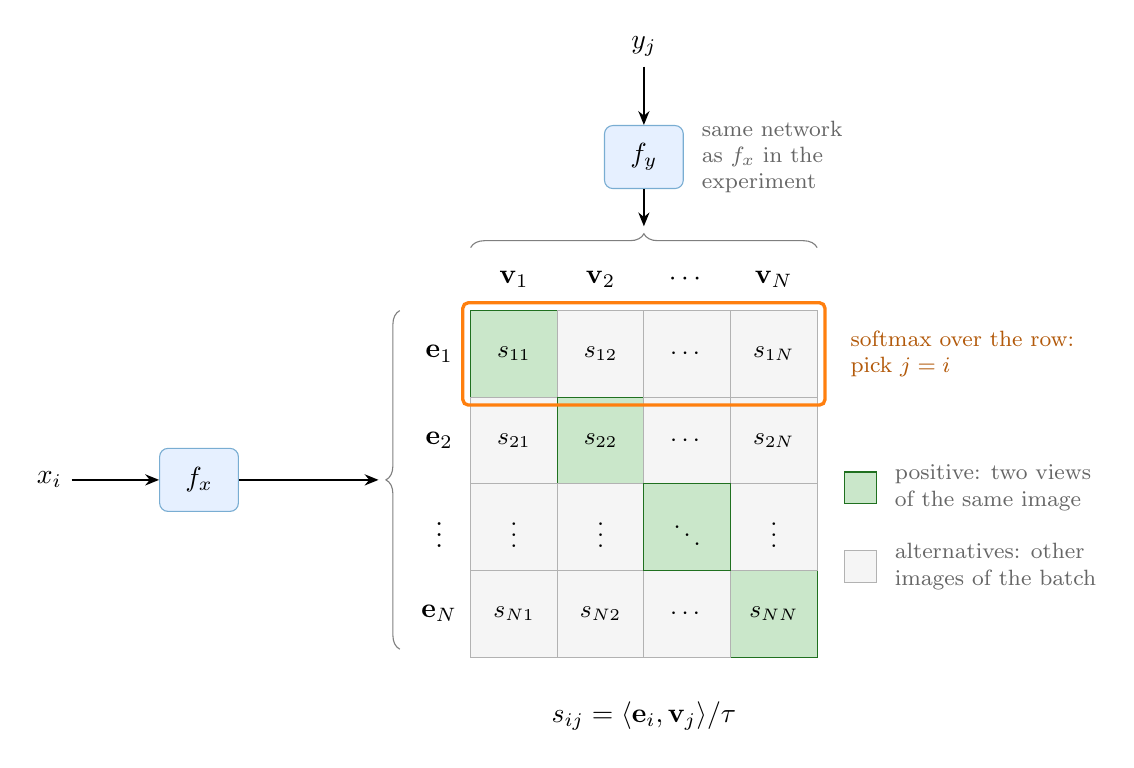
\begin{tikzpicture}[
  cell/.style={draw=aux!60, minimum size=1.1cm, inner sep=0pt, font=\small},
  positive/.style={cell, fill=msg!25, draw=msg!70!black},
  alternative/.style={cell, fill=aux!8},
]

% === Score matrix: row i is x_i (vector e_i), column j is y_j (vector v_j) ===
% Cell (i,j) sits at x = (j-1)*1.1, y = -(i-1)*1.1. Index 3 stands for the omitted ones.
\foreach \i/\a in {1/1,2/2,4/N}{
  \foreach \j/\b in {1/1,2/2,4/N}{
    \ifnum\i=\j
      \node[positive] at ({(\j-1)*1.1},{-(\i-1)*1.1}) {$s_{\a\b}$};
    \else
      \node[alternative] at ({(\j-1)*1.1},{-(\i-1)*1.1}) {$s_{\a\b}$};
    \fi
  }
}
\foreach \k in {1,2,4}{
  \node[alternative] at ({2*1.1},{-(\k-1)*1.1}) {$\cdots$};
  \node[alternative] at ({(\k-1)*1.1},{-2*1.1}) {$\vdots$};
}
\node[positive] at ({2*1.1},{-2*1.1}) {$\ddots$};

% === Labels: unit vectors of each side ===
\foreach \j/\b in {1/1,2/2,4/N}{
  \node at ({(\j-1)*1.1},0.95) {$\mathbf{v}_{\b}$};
  \node at (-0.95,{-(\j-1)*1.1}) {$\mathbf{e}_{\b}$};
}
\node at ({2*1.1},0.95) {$\cdots$};
\node at (-0.95,{-2*1.1}) {$\vdots$};

% === Encoder f_y (columns) ===
\node (y) at (1.65,3.9) {$y_j$};
\node[encoder] (fy) at (1.65,2.5) {$f_y$};
\draw[flow] (y) -- (fy);
\draw[decorate, decoration={brace, amplitude=5pt}, draw=aux] (-0.55,1.35) -- (3.85,1.35);
\draw[flow] (fy) -- (1.65,1.62);
\node[annotation, right=3pt of fy, align=left] {same network\\as $f_x$ in the\\experiment};

% === Encoder f_x (rows) ===
\node (x) at (-5.9,-1.6) {$x_i$};
\node[encoder] (fx) at (-4.0,-1.6) {$f_x$};
\draw[flow] (x) -- (fx);
\draw[decorate, decoration={brace, amplitude=5pt}, draw=aux] (-1.45,-3.75) -- (-1.45,0.55);
\draw[flow] (fx) -- (-1.72,-1.6);

% === Softmax over the row of the positive ===
\draw[highlight, line width=1.2pt, rounded corners=2pt]
  (-0.65,-0.65) rectangle (3.95,0.65);
\node[right, align=left, font=\footnotesize, text=highlight!70!black]
  at (4.15,0) {softmax over the row:\\pick $j=i$};

% === Legend ===
\node[positive, minimum size=0.4cm] (lp) at (4.4,-1.7) {};
\node[annotation, right=3pt of lp, align=left] {positive: two views\\of the same image};
\node[alternative, minimum size=0.4cm] (la) at (4.4,-2.7) {};
\node[annotation, right=3pt of la, align=left] {alternatives: other\\images of the batch};

% === Score ===
\node at (1.65,-4.6) {$s_{ij}=\langle\mathbf{e}_i,\mathbf{v}_j\rangle/\tau$};

\end{tikzpicture}
\end{document}
